\section{Datenbank}

Daten werden mithilfe von \href{https://pub.dev/packages/isar}{Isar} persistiert. In Bild \ref{img:erm} ist ein ERM-Diagramm der Datenbank abgebildet.
Auch wenn innerhalb der Zugriffe auf Isar mit speziellen Datenklassen gearbeitet wird, wandeln die DAOs diese beim Zugriff in die
Model-Klassen der MVC-Schicht um. So werden zum Beispiel die Events direkt in die enthaltene Liste der \verb|SingleItem|-Klasse eingefügt und nicht seperat angefragt.

Bilder werden im Dokumenten-Verzeichnis der Anwendung abgelegt und in der Datenbank nur der dazugehörige Pfad gespeichert.

\begin{figure}[H]
  \centering
  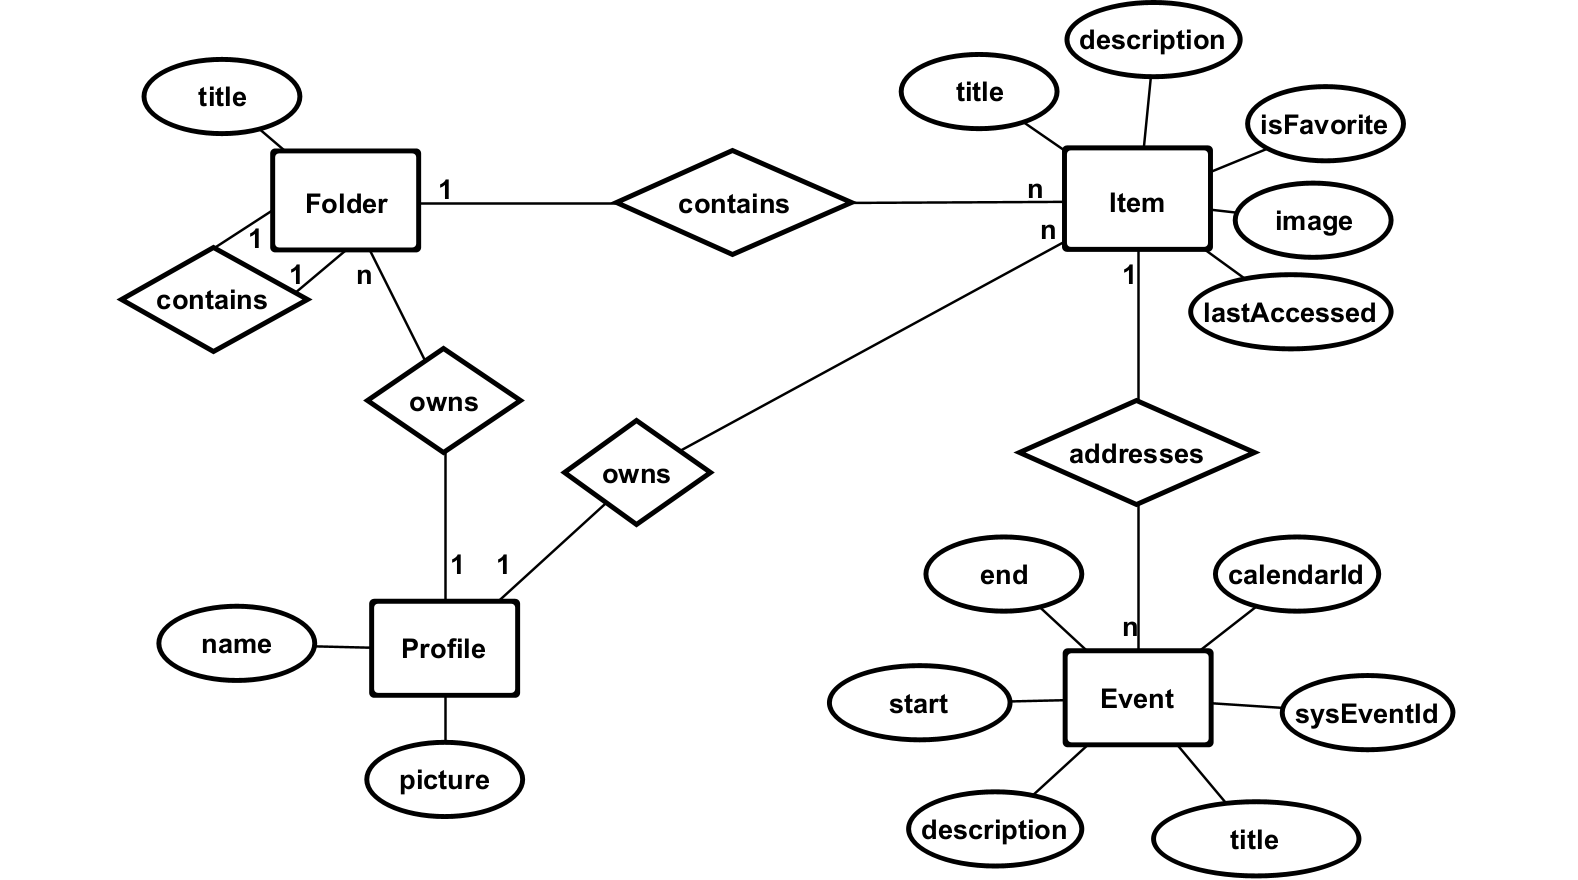
\includegraphics[width=0.8\textwidth]{figures/persistenz_erm.png}
  \caption{Persistenz ERM Diagram}
  \label{img:erm}
\end{figure}

Eine technische Besonderheit sind die Profile. Profile erlauben dem Nutzer, Daten noch einmal grober zu kategorisieren als Ordner.
Um dies umzusetzen, verwaltet Isar ebenfalls eine Tabelle für Profile. Jeder andere Eintrag der Datenbank wird dann einem Profil zugeordnet.
Die Besonderheit besteht darin, dass beim erstmaligen Starten der App ein Standard-Profil angelegt wird, welches zudem als eine globale Sicht fungiert.
Das bedeutet, wenn ein Nutzer weitere Profile anlegt und mit Daten füllt, sind diese Daten auch über das Standard-Profil sichtbar.
Zudem funktioniert die App auch ohne weitere Profile und es ändert sich nichts an der Nutzung, wenn ein Nutzer keine Profile erstellen möchte.
Das derzeit ausgewählte Profil ist über den Provider für die App-Einstellungen erhältlich. Auf diesen wird beim erstellen des PersistenceProviders ein \verb|watch| ausgeführt.
Dadurch erhält jeder Controller automatisch einen PersistenceService, in dem das aktuelle Profil vermerkt ist, sodass die richtigen Daten zurückgeliefert werden.

Funktionalitäten zum Verschieben von Inhalten zwischen Profilen aber auch zwischen Ordnern sind im Backend bereits implementiert, allerdings sind diese noch
nicht über die View zugreifbar.

\section{Einstellungen}

Um die Einstellungen, die ein Nutzer vornehmen kann, zu speichern, wird das Plugin \href{https://pub.dev/packages/shared_preferences}{shared\_preferences} genutzt.
Dabei speichern wir zum Beispiel den ausgewählten System-Kalendar, das ausgewählte Farbschema, Profil und Sprache. Diese werden, wie üblich über einen per Riverpod verfügbaren Provider abgerufen.
